\begin{frame}{工作总结}
工作量:
\begin{itemize}
\item Vit2019: 目前最大的白癜风分割数据集
\item 大量的实验验证
\item 撰写论文和专利
\end{itemize}

\vspace{0.1cm}

创新点:
\begin{itemize}
\item 基于显著性传播的弱监督分割方法:
\begin{itemize}
\item 应用超像素技术
\item ``既见树木,又见森林''策略
\item 将反馈思想与显著性传播相结合
\end{itemize}
\end{itemize}

\vspace{0.1cm}

其他工作:
\begin{itemize}
\item 集成分割算法到皮研所系统
\end{itemize}

\vspace{-0.2cm}

\begin{figure}
    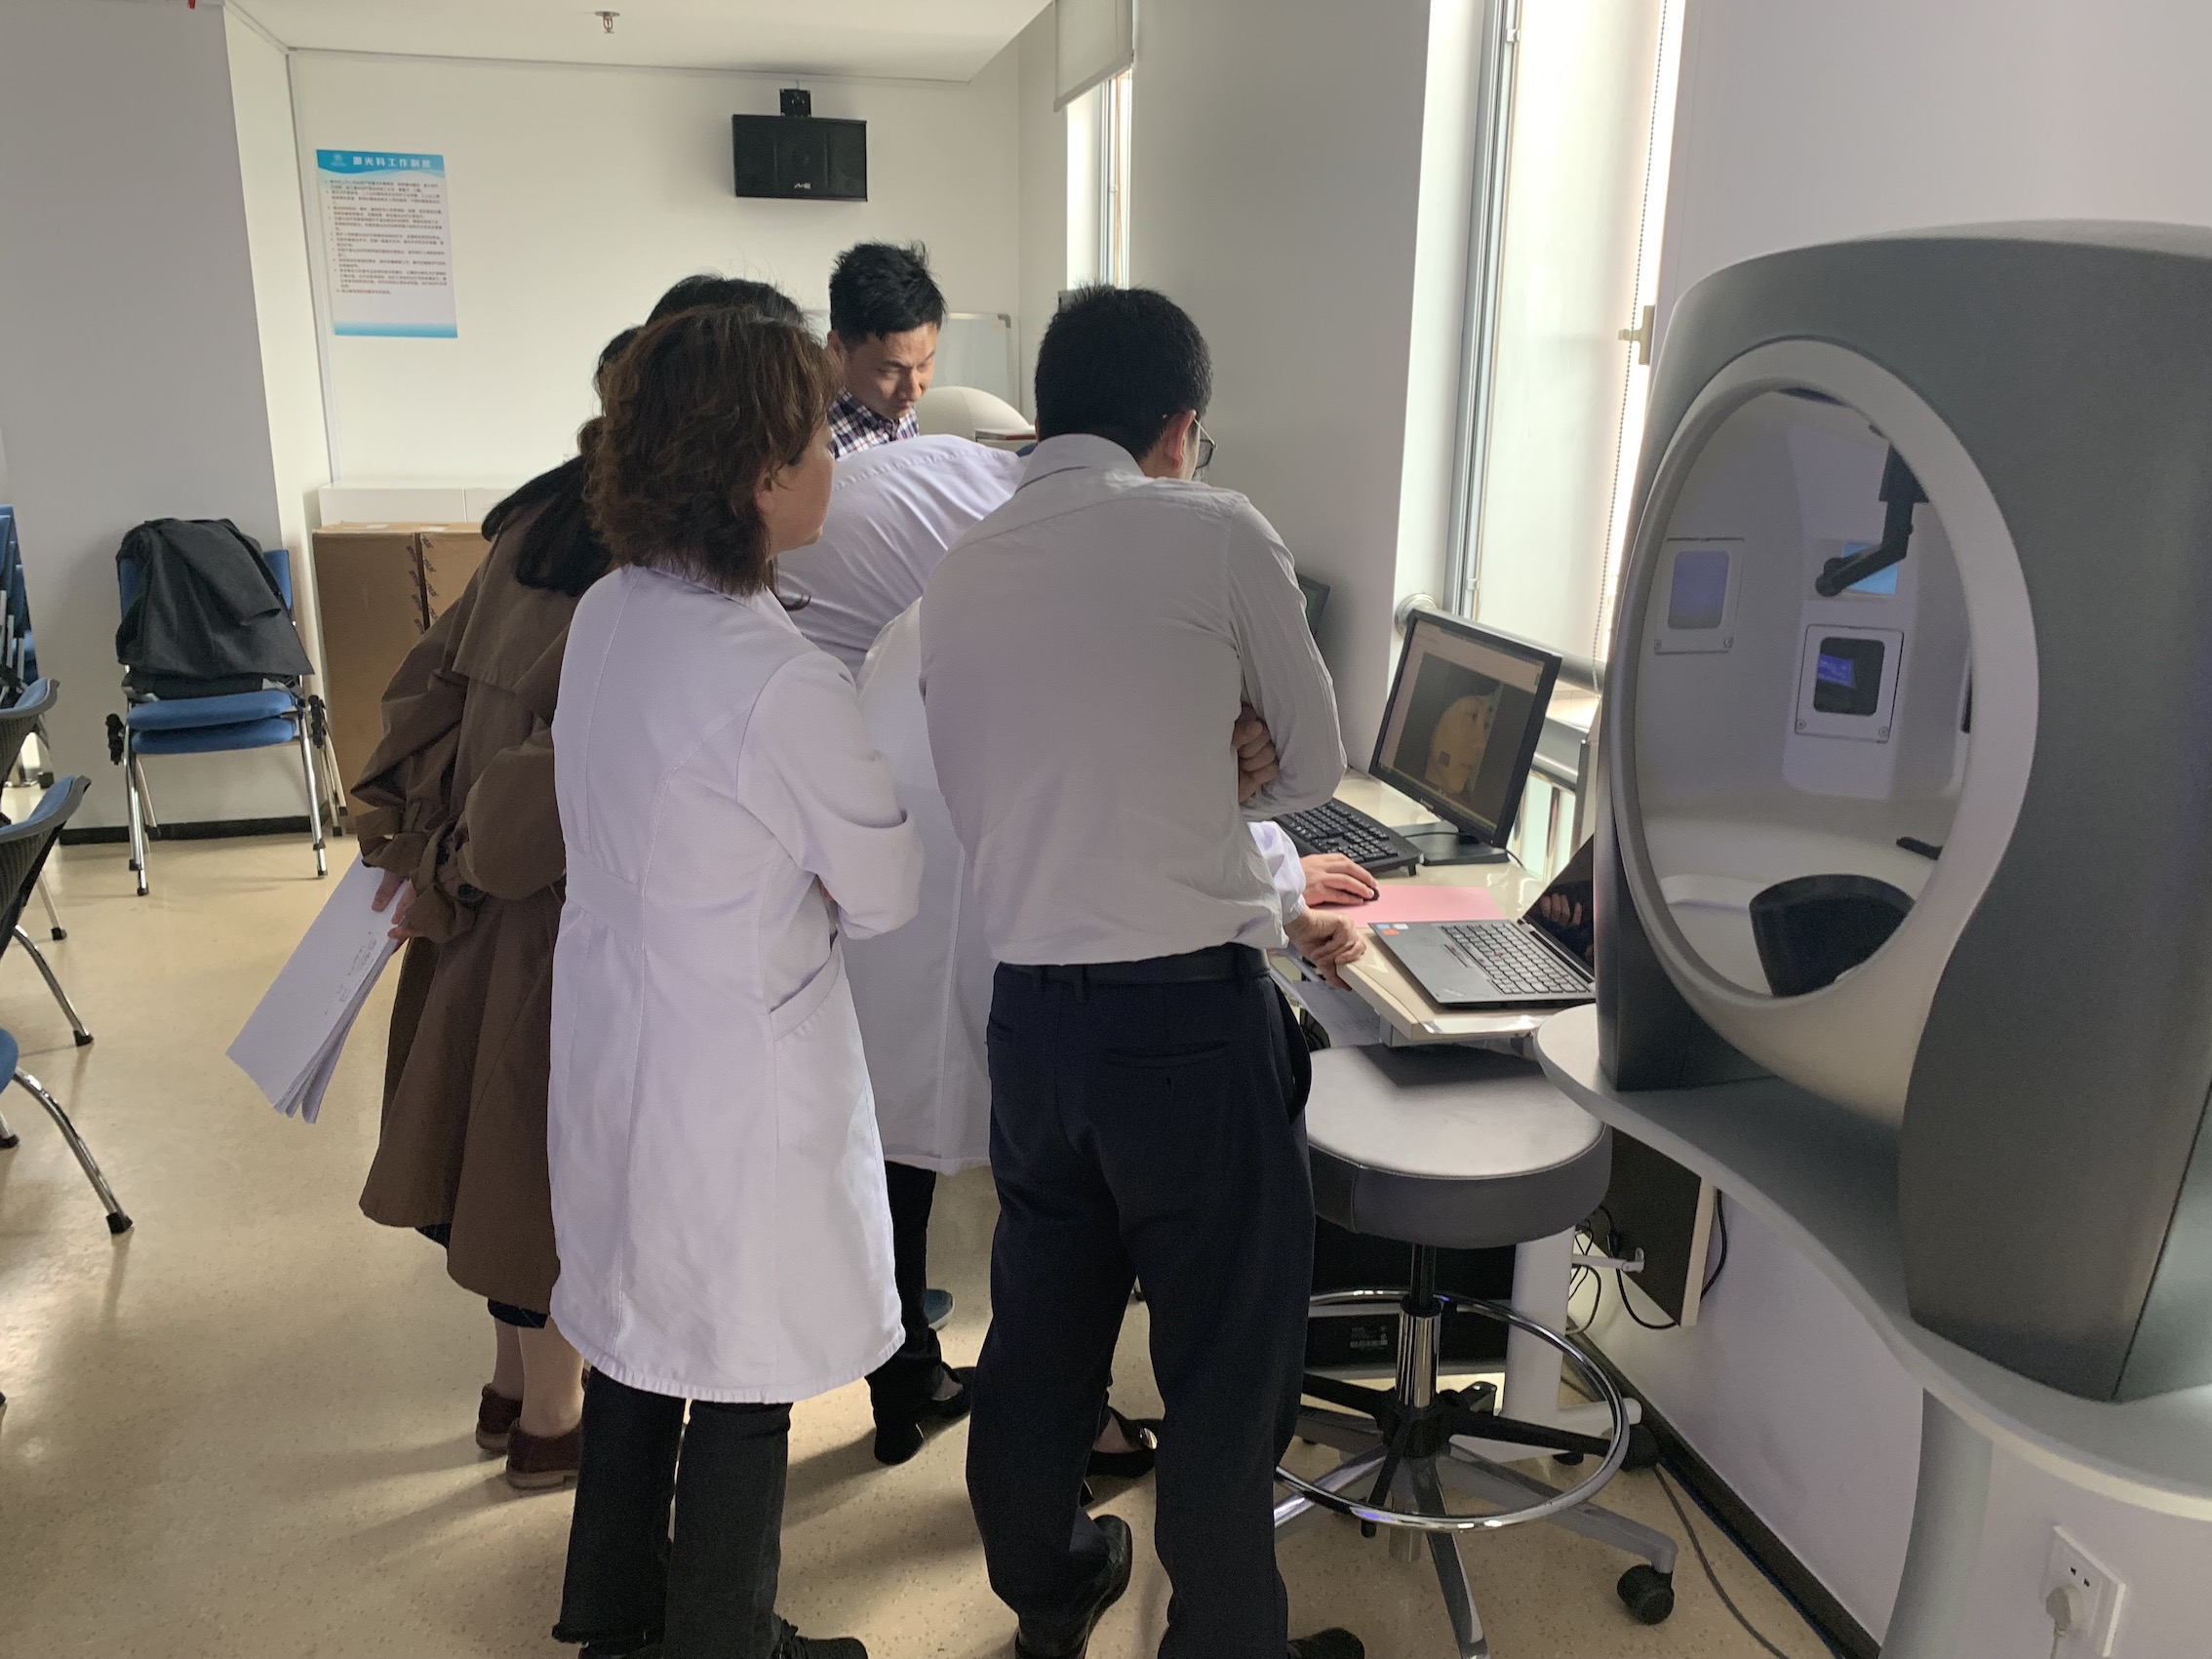
\includegraphics[width=.26\linewidth]{figures/presentation2.jpg}
    \hspace{0.05cm}
    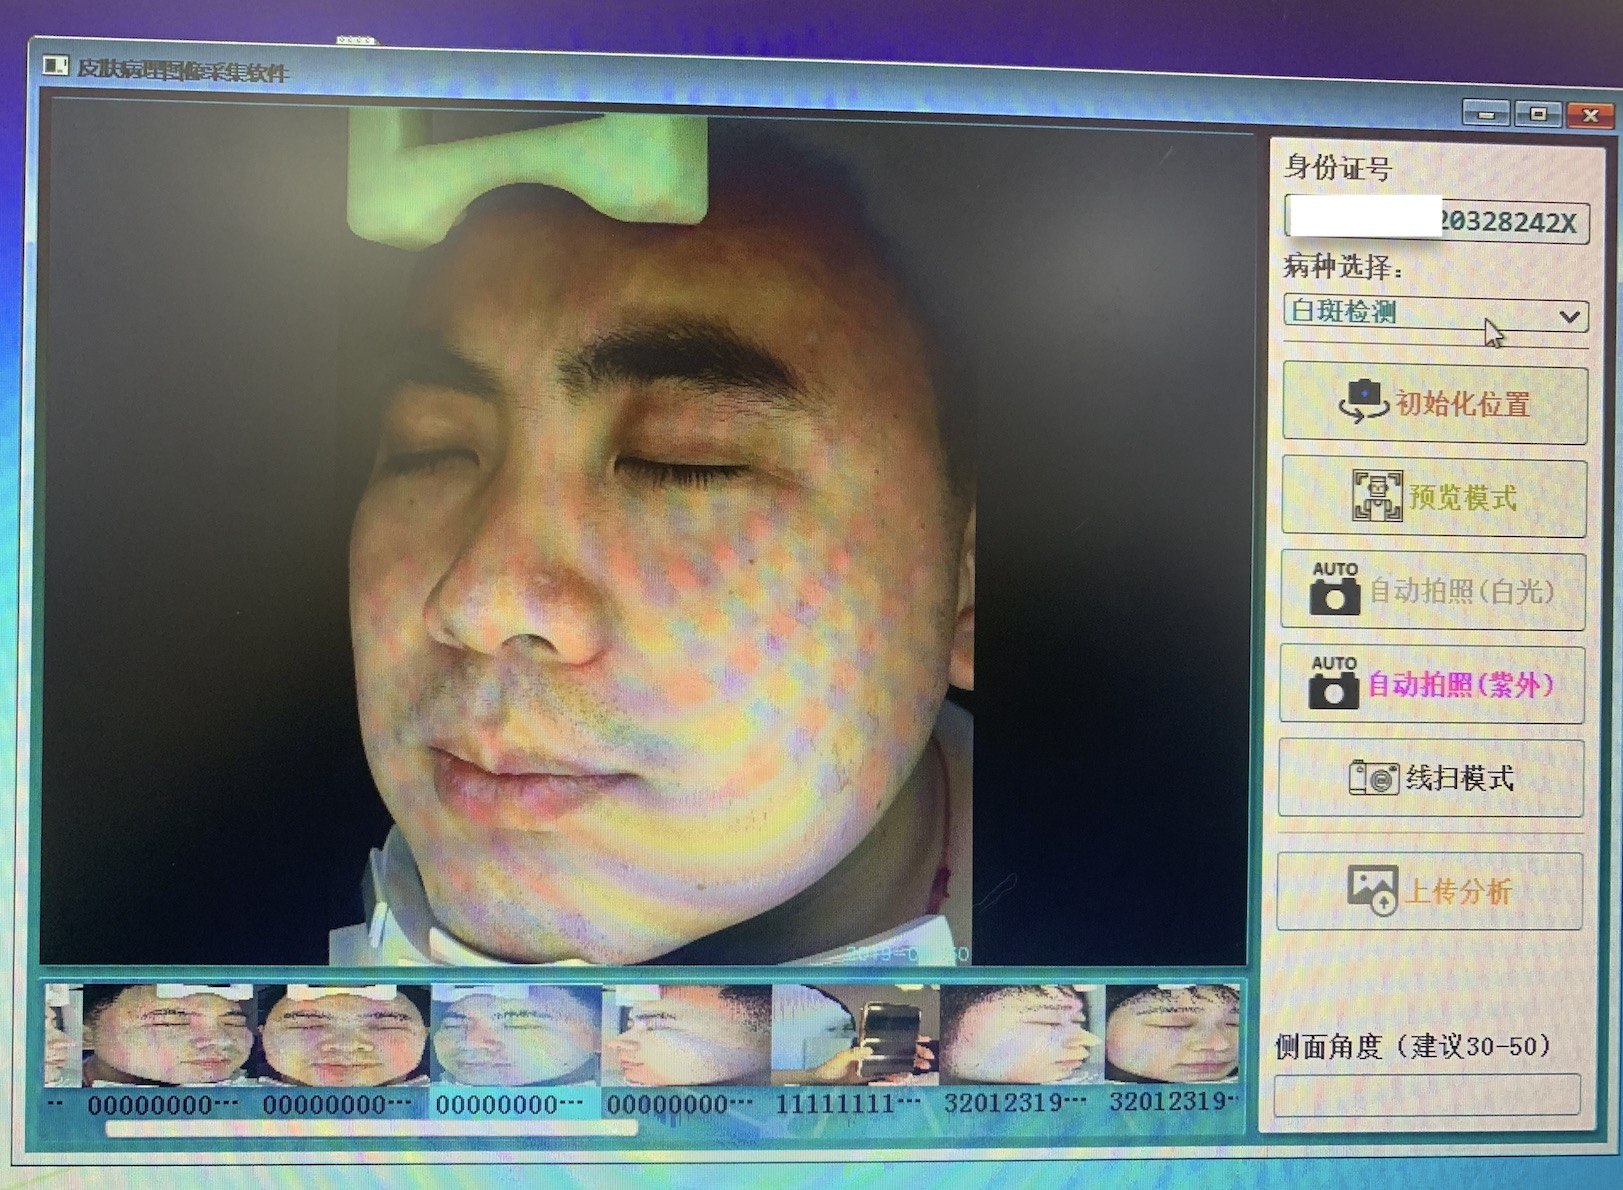
\includegraphics[width=.26\linewidth]{figures/presentation1.jpg}
\end{figure}
\end{frame}
%其他工作:
%\begin{columns}
%\column{.5\textwidth}
%\begin{itemize}
%\item 集成分割算法到皮研所系统
%\end{itemize}
%\column{.5\textwidth}
%\begin{figure}
%    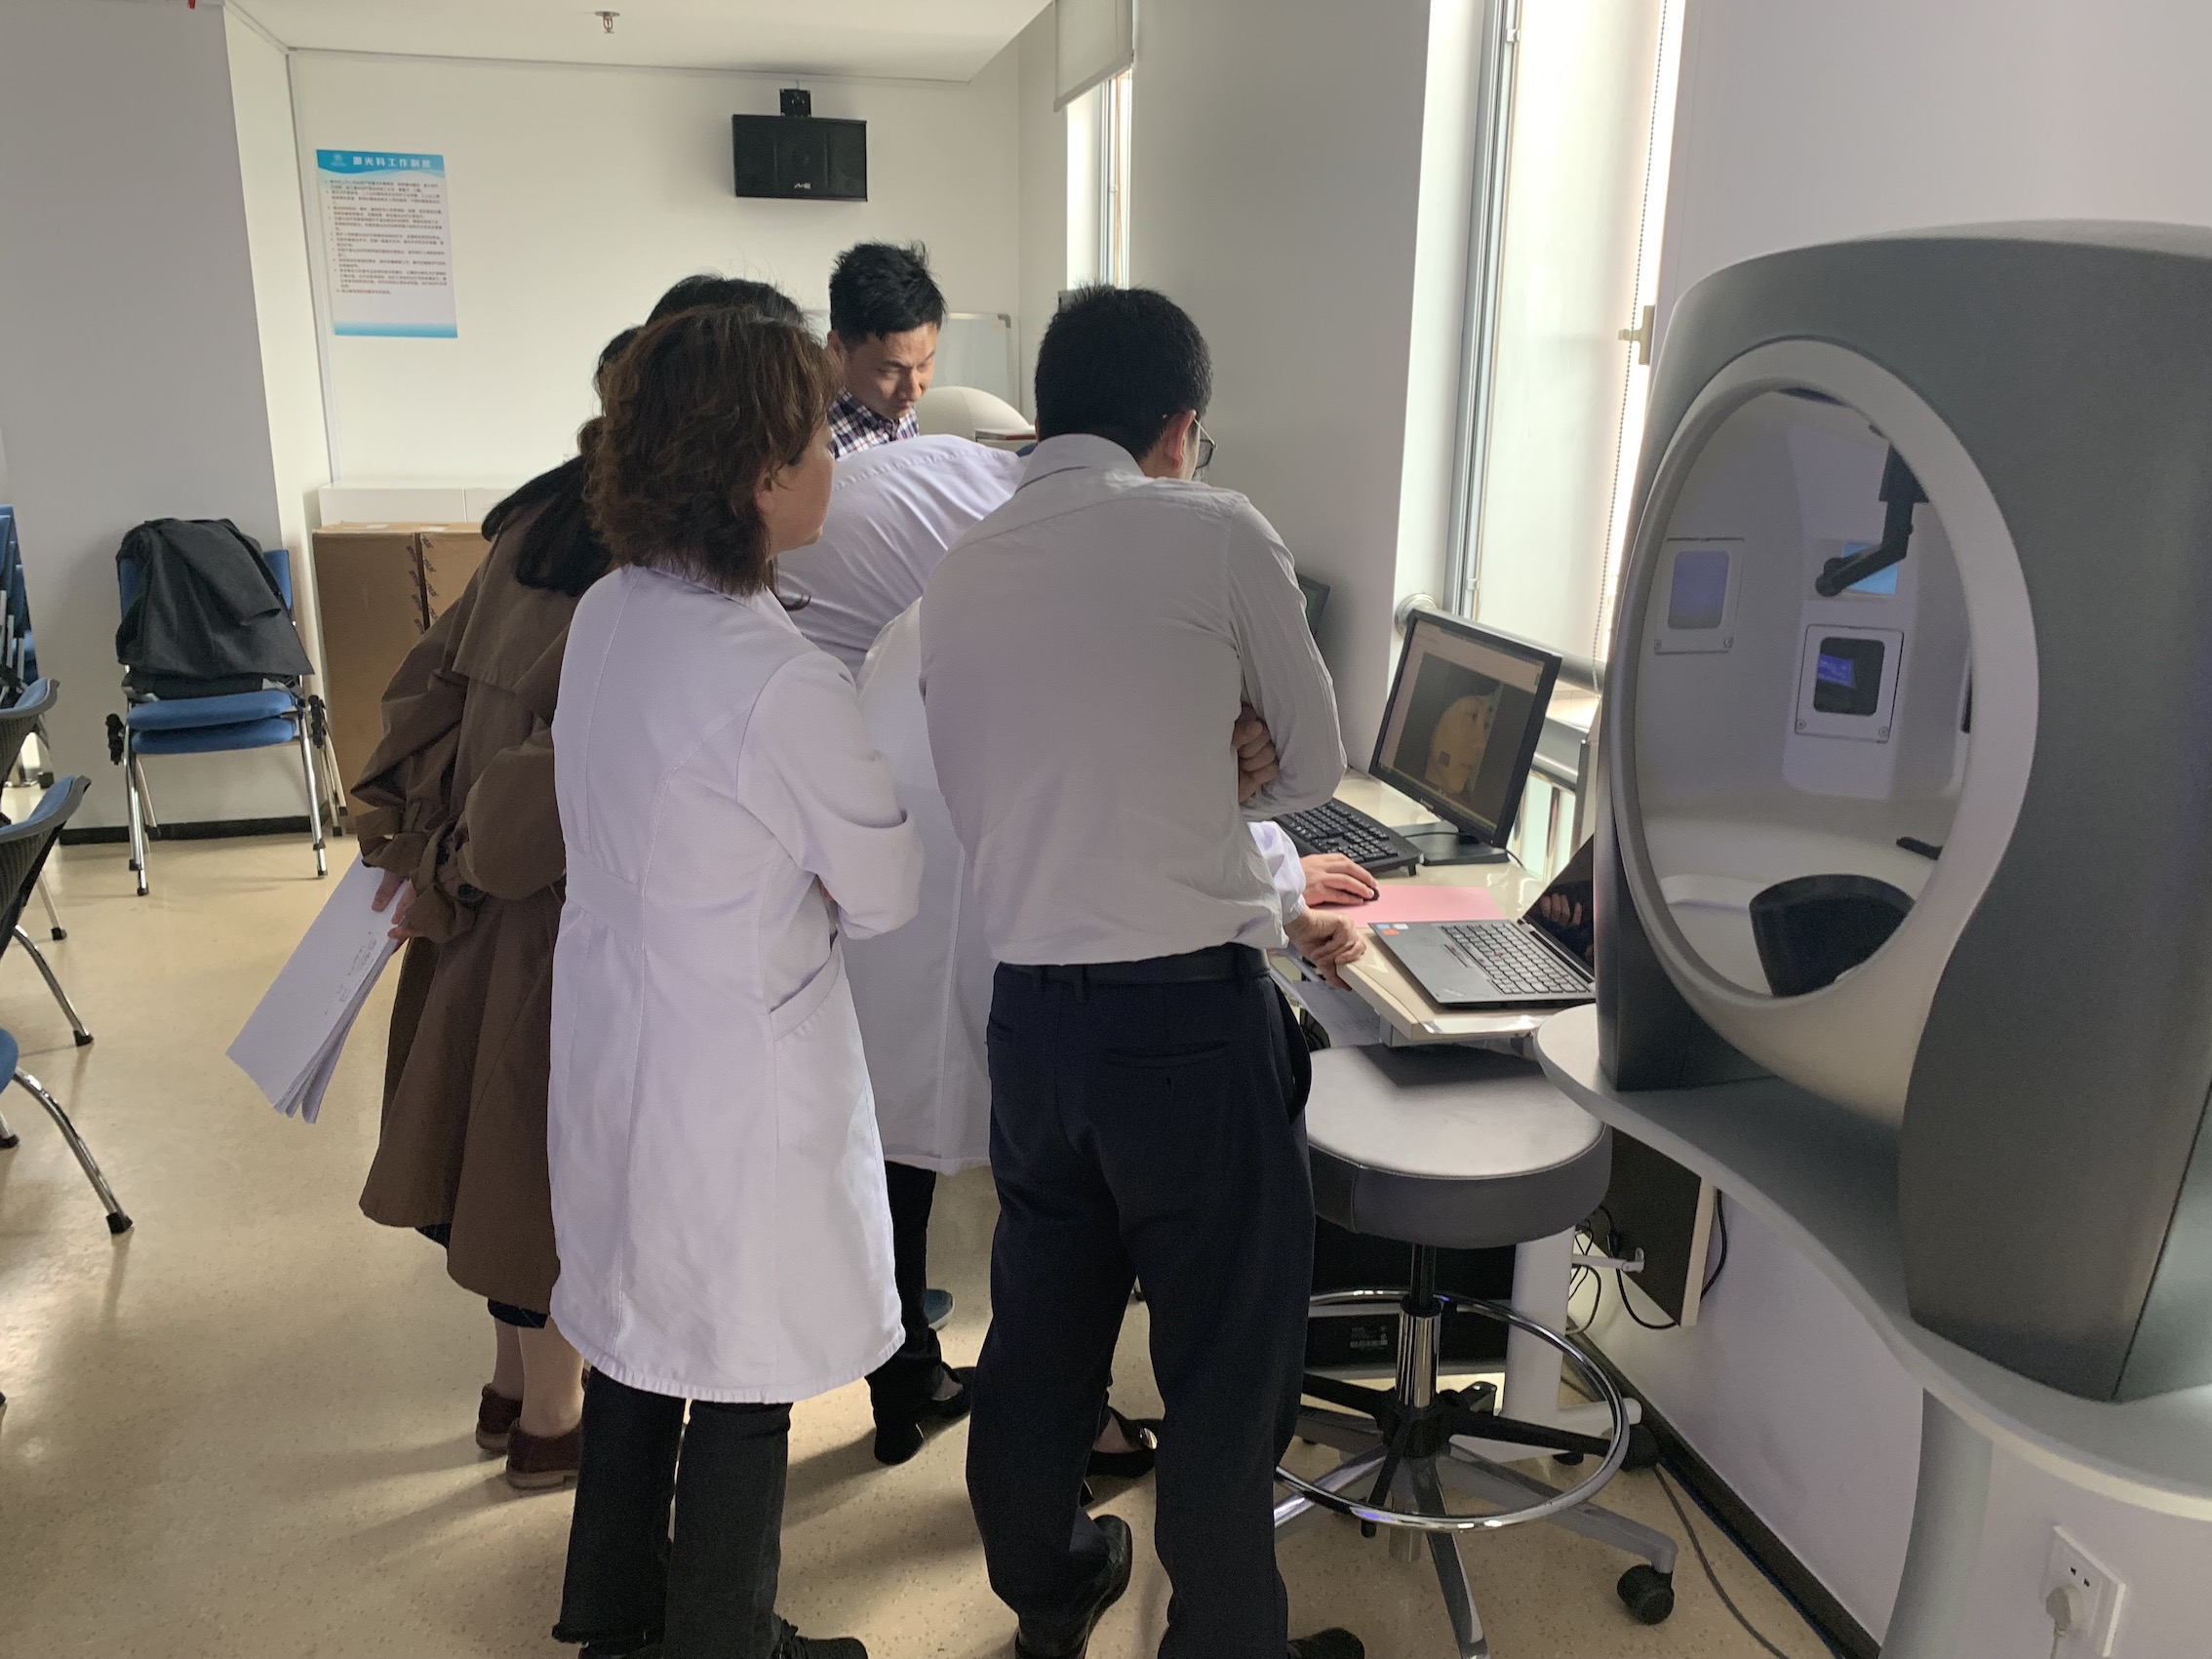
\includegraphics[width=.48\linewidth]{figures/presentation2.jpg}
%    \hspace{0.05cm}
%    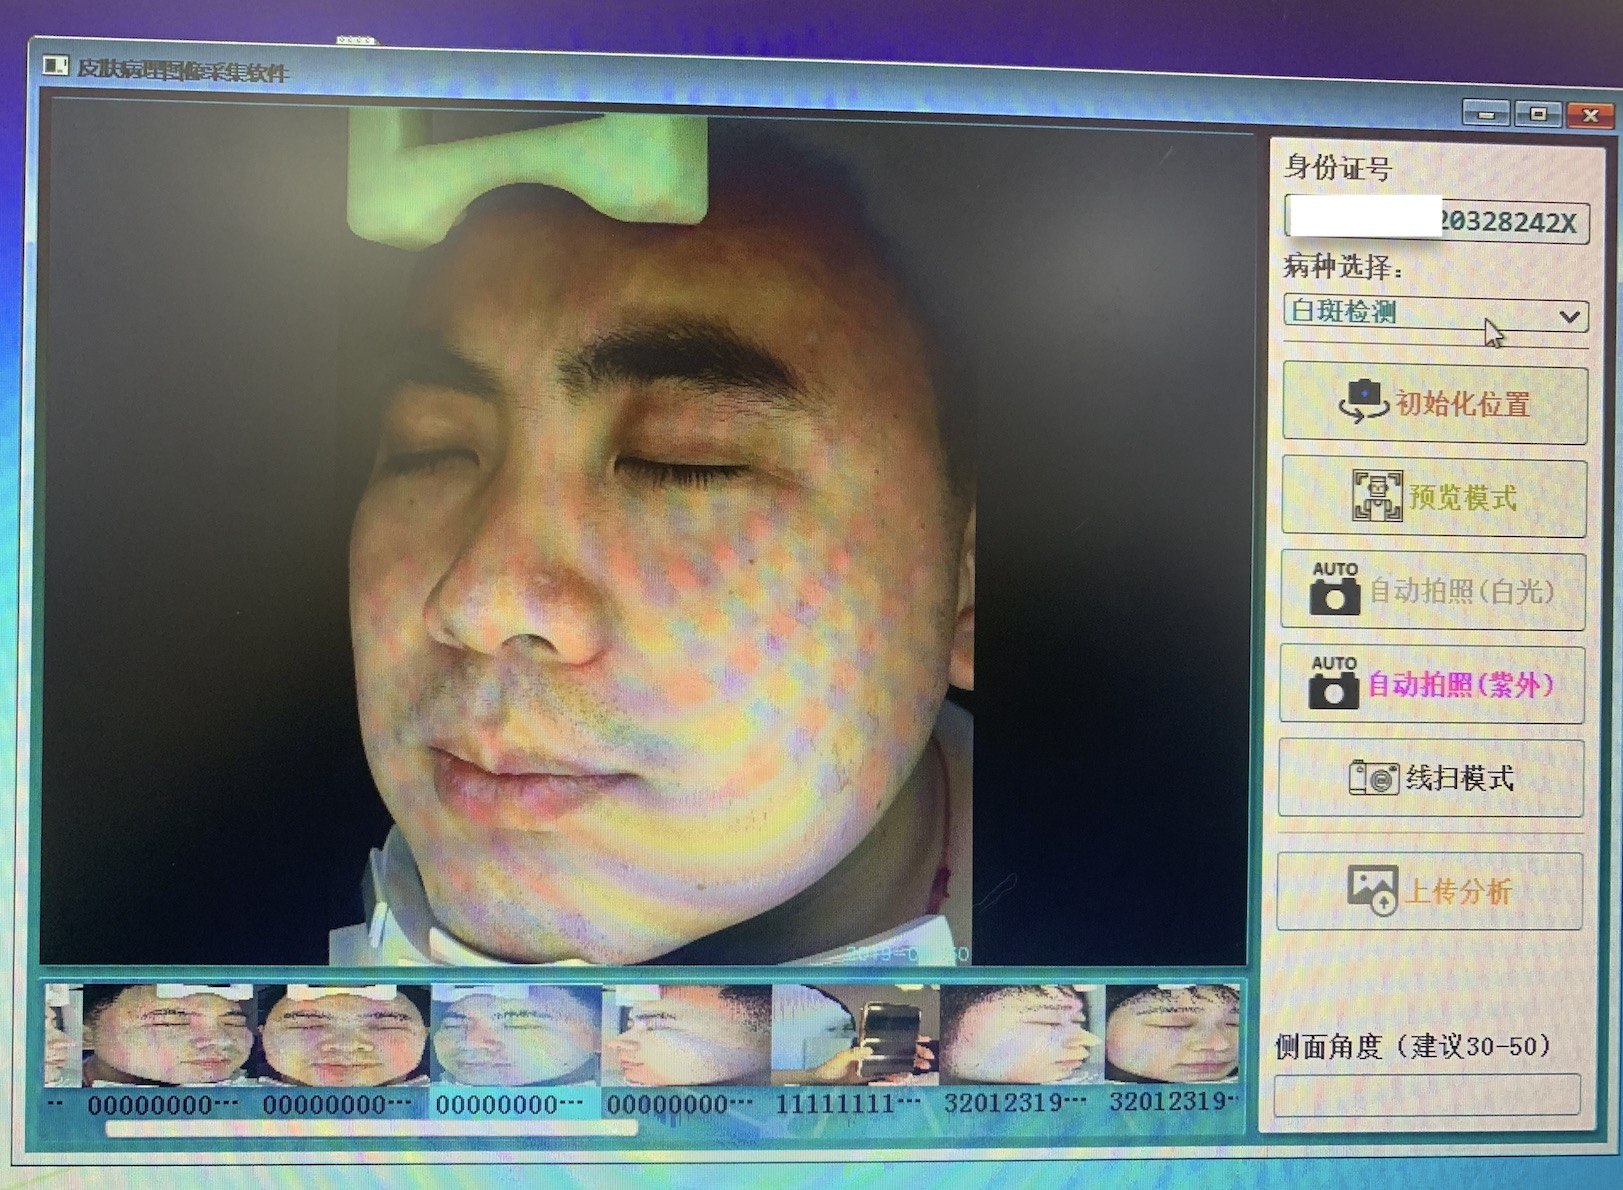
\includegraphics[width=.48\linewidth]{figures/presentation1.jpg}
%\end{figure}
%\end{columns}


%%%
\begin{frame}{工作总结}
论文\footnote{\tiny \textbf{Zhangxing Bian, Siyu Xia}, Chao Xia, Ming Shao, FU YUN. Weakly Supervised Vitiligo
Segmentation in Skin Image through Saliency Propagation.\textit{In Proceedings of the IEEE
international conference on computer vision, 2019}}(于3月投稿ICCV\footnote{\tiny 计算机视觉领域三大顶会之一})
\hspace{2.5cm}专利\footnote{\tiny 发明人:\textbf{边张行, 夏思宇}; 公布号:CN 109741336 A}(已公开)
\begin{figure}
    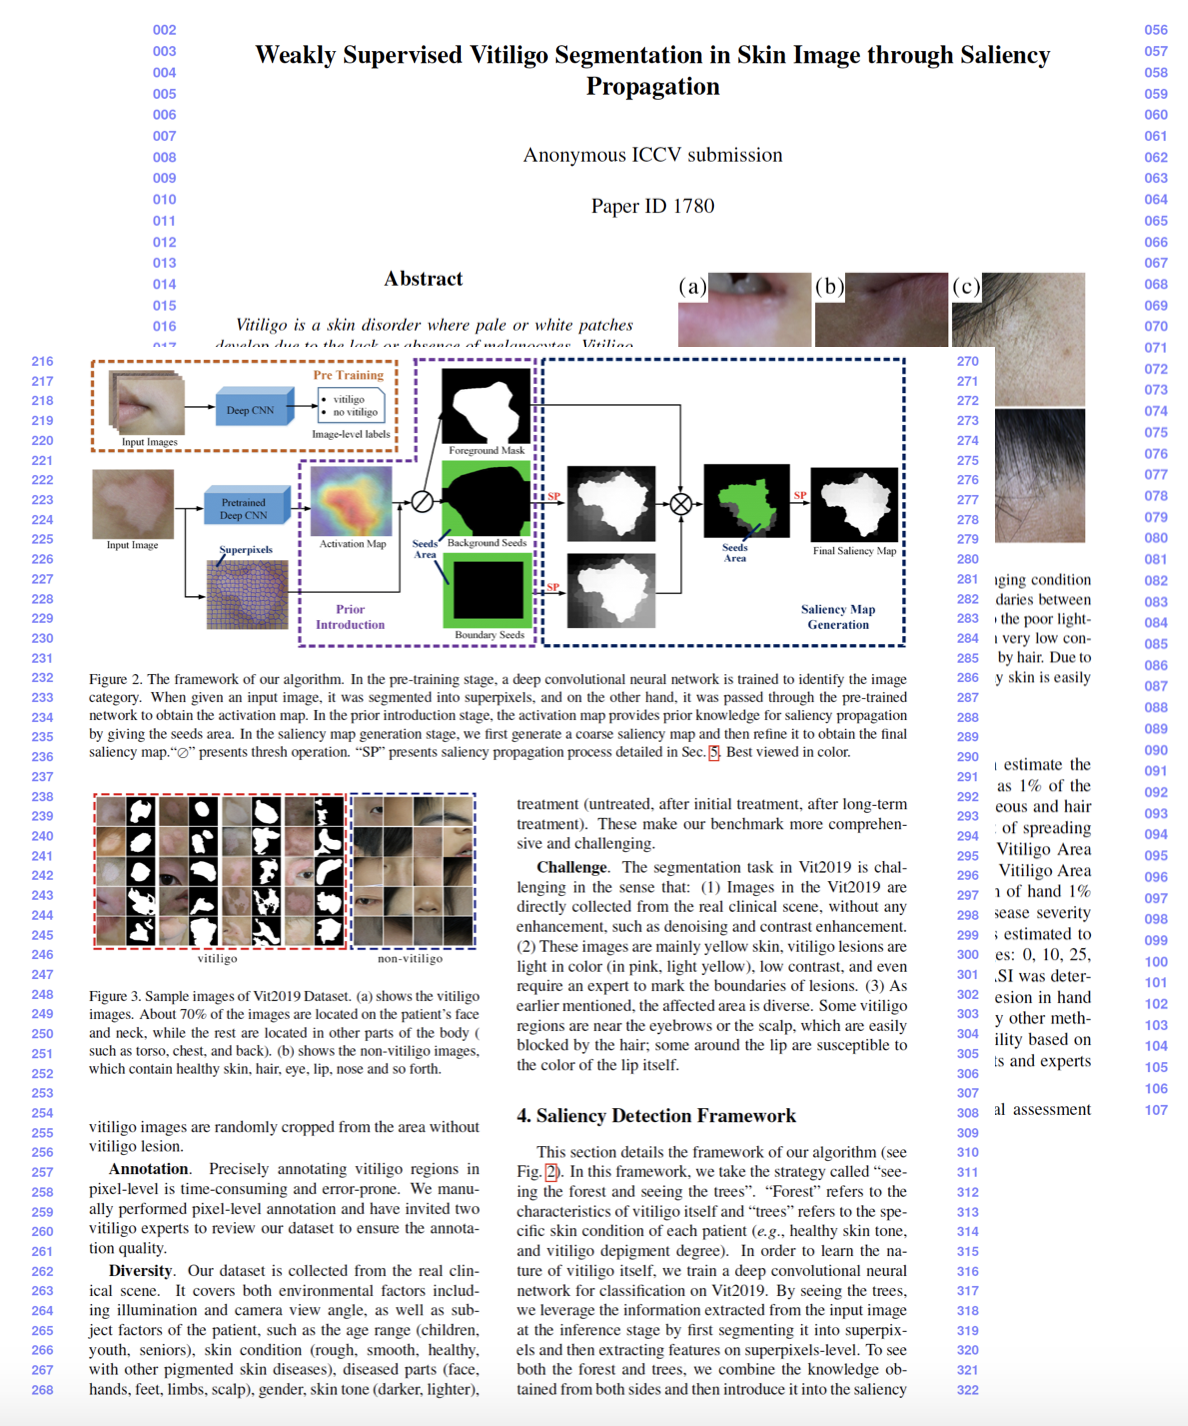
\includegraphics[width=.4\linewidth]{figures/paperFigure.png}
    \hfill
    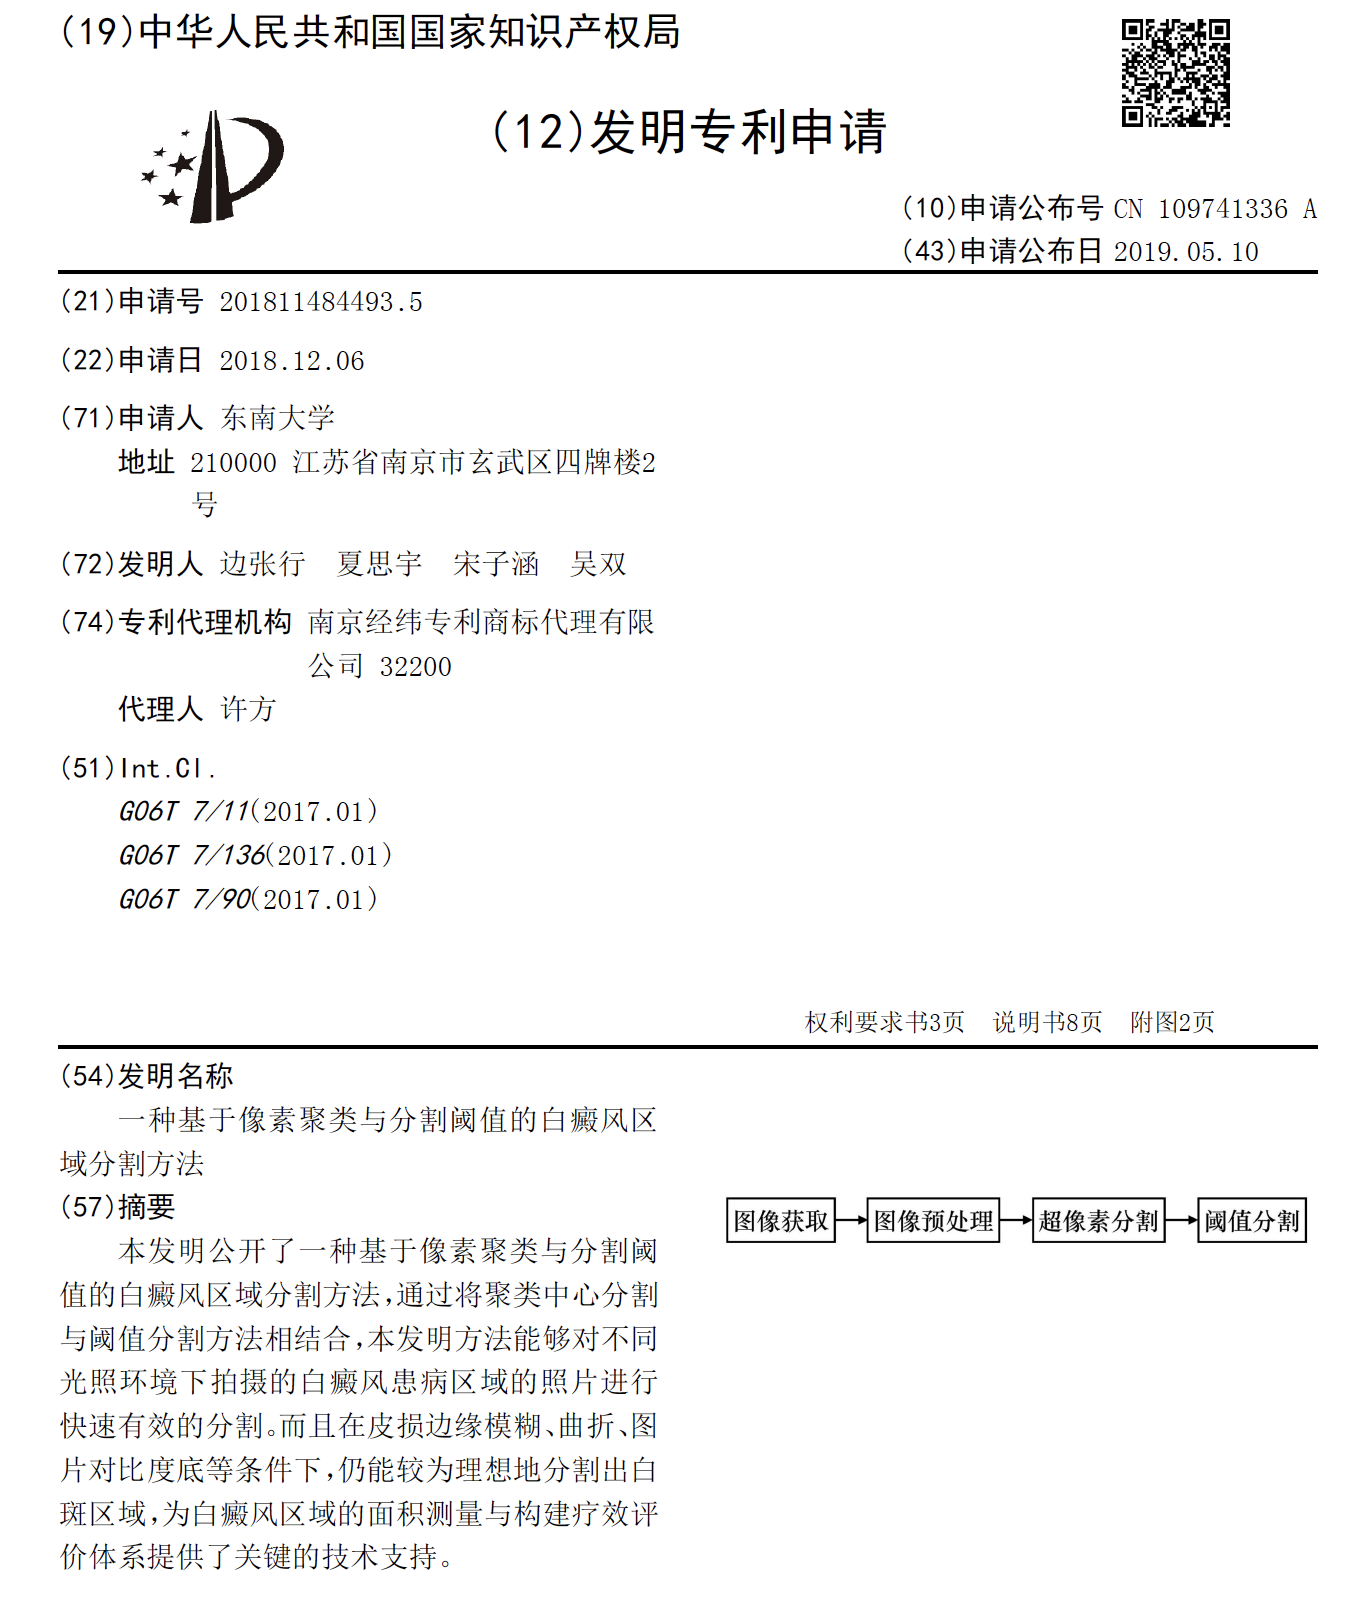
\includegraphics[width=.4\linewidth]{figures/patent.png}
\end{figure}
\end{frame}
%%%
\begin{frame}{展望}
\begin{itemize}
\item 应用:弱监督分割+交互式标注
\item 应用:其他皮损区域的分割 e.g. 黄褐斑、雀斑、烧伤
\begin{figure}
    
\includegraphics[width=.6\linewidth]{figures/meldemo.png}
\end{figure}

\item 计算皮损区域的绝对物理面积~$\Rightarrow$~3D人脸模型
\end{itemize}

\begin{figure}
    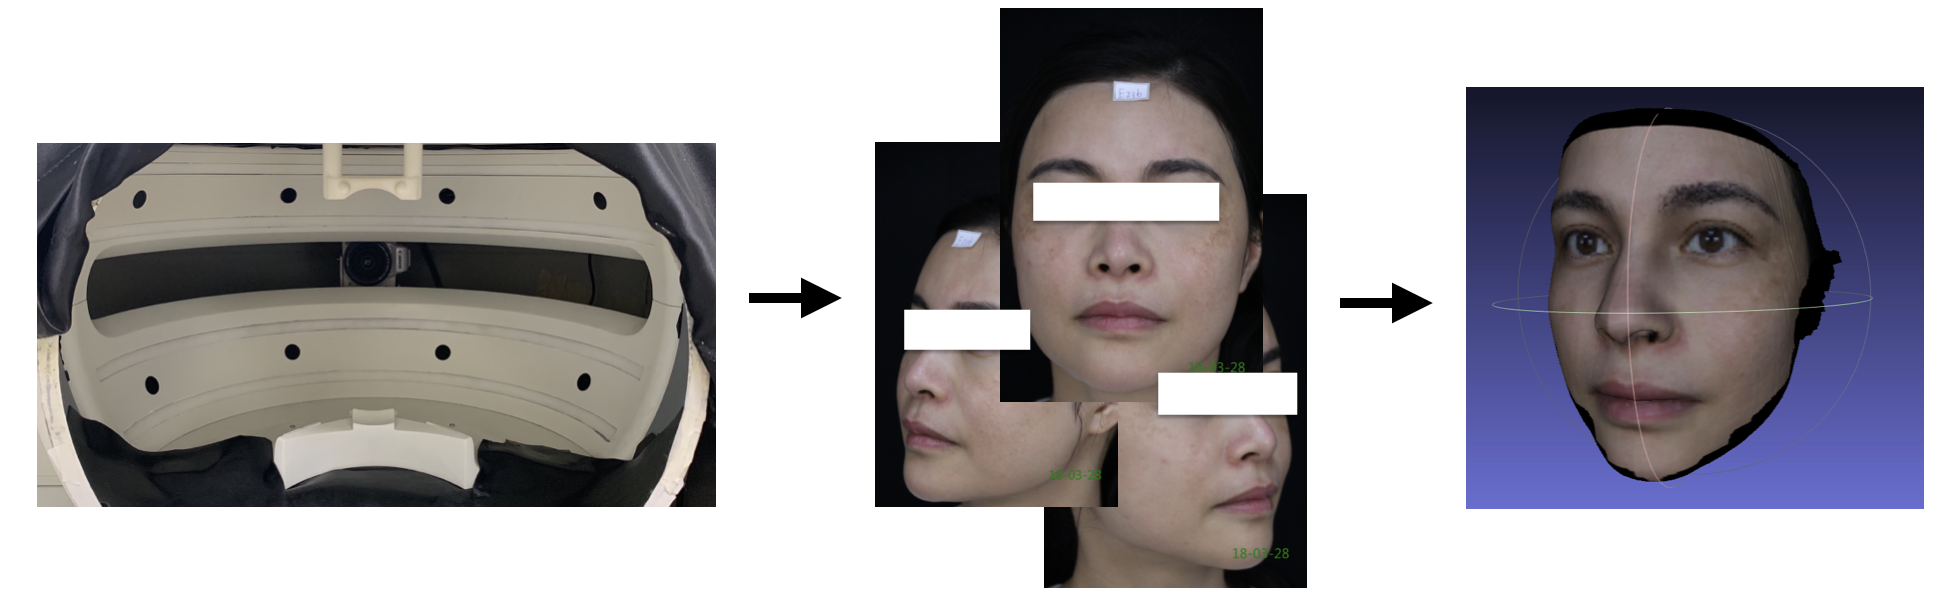
\includegraphics[width=.9\linewidth]{figures/statCamera.png}
\end{figure}

\end{frame}


\begin{frame}{}
\centering \huge
致谢

\vspace{.8cm}

\Large
感谢{\color{blue}{夏思宇}}老师!

\vspace{.4cm}

感谢{\color{blue}{钱堃}}、{\color{blue}{王雁刚}}、{\color{blue}{王辰星}}老师在相关领域给与的启发和帮助!

\vspace{.4cm}

感谢各位评审老师的聆听!
\end{frame}

















